\documentclass[
    oneside,
    11pt,
    a4paper
]{utad_msc}

% Packages
\usepackage[autostyle=true]{csquotes}
\usepackage{lmodern} % Support latin modern fonts
\usepackage[T1]{fontenc} % Support for T1 enconding
\usepackage[spanish,activeacute]{babel} % Set spanish language
\usepackage[autostyle=true]{csquotes}
\usepackage{mathtools} % Add additional tools for math writing 

\makeatletter
\renewcommand{\frontmatter}{\cleardoublepage\@mainmatterfalse}
\renewcommand{\mainmatter}{\cleardoublepage\@mainmattertrue}
\makeatother

\graphicspath{ {./images/} }
\setcounter{tocdepth}{4}
\setcounter{secnumdepth}{4}

\student{Anxo Babío Rodríguez}
\tutor{Iván Alduán Íñiguez}
\course{Máster en computación gráfica realidad virtual y la simulación}
\project{Materiales PBR en WebGL 2.0}


\AtBeginDocument{%
  \addtocontents{toc}{\protect\thispagestyle{empty}}
}

\begin{document}
    \begin{titlepage}
    \newgeometry{left=2cm,bottom=2cm, top=3.5cm, right=2cm}
    \begin{figure*}
        
\includegraphics[scale=1]{logo_ucjc}\hfill%
        
\includegraphics[scale=1]{logo_utad}%
        \vspace{1cm}
    \end{figure*}
    \title{
        \large \MakeUppercase{\utadcourse} \\
        \vspace{0.5cm}
        \Huge \MakeUppercase{\utadtitle}
        \vfill
    }
    \author{
        AUTOR: \MakeUppercase{\utadstudent} \\
        TUTOR: \MakeUppercase{\utadtutor}
    }
    \date{}
    \maketitle
\end{titlepage}
    \begingroup
      \pagestyle{plain}
      \tableofcontents
      \listoffigures
    \endgroup
    \clearpage

    \pagestyle{fancy}
    \frontmatter
      \chapter{Marco colaborativo}
Seddi es una startup nacida como fruto de la investigacion en tecnologias de simulacion optica y mecanica aplicadas al sector textil.
Propone ofrecer una solucion digital que permita a los disenhadores, patronistas o comerciales trabajar en un entorno colaborativo que
representa con gran fidelidad los elementos constructivos de un prenda de ropa: tejido, costuras, dobladillos, etc.

La caida, el brillo y, en general, la apariencia de una prenda son factores clave para validar o rechazar el producto, estas caracteristicas
dependen de propiedades opticas y mecanicas que las herramientas de disenho actuales no tienen en cuenta, por lo que los profesionales del
sector no satisfacen las necesidades de los profesionales de la industria, que en la mayor parte de los casos mantienen un proceso de
trabajo artesanal en el que el prototipado y construccion de la prenda es un proceso iterativo entre patronista y disenhador y cuyo
resultado depende en gran medida de la experiencia y destreza de estos profesionales.

Para ofrecer su solucion, Seddi cuenta con departamentos de investigacion simulacion y captura tanto mecanica como optica, que desarrollan
nuevos algoritmos y hardware que permitan un mayor grado de fidelidad en el momento de captura de los parametros que conforman la apariencia
de una prenda, tanto como mejorar su representacion digital asi como departamentos de desarrollo de producto, se encargan del proceso de
captura utilizando estas tecnologias propietarias asi como de integrar estos algoritmos en diferentes plataformas que permitan al consumidor
final interactuar sobre los tejidos digitales durante diferentes etapas asociadas a este proceso de produccion con el fin de facilitar,
acelerar y reducir los costes de produccion.

Para conseguir un resultado fidedigno, en Seddi, el proceso comienza creando un clon digital del tejido, la obtencion de parametros opticos y
mecanicos que identifican el tejido y se valida utilizando las tecnologias de simulacion y render de la empresa. 

Todos las herramientas de Seddi se alojan en la nube, lo que garantiza disponibilidad inmediata a los recursos a todo el equipo involucrado en
el proceso de produccion. Estos equipos, con un negocio de la moda cada dia mas globalizado, pueden tratarse de equipos multidisciplinares de
diferentes empresas o paises, por lo que es primordial un flujo de comunicacion constante que minimice los errores y los costes economicos y
medioambientales de los flujos de disenho y prototipado

Gracias a esta estrategia de implementación, el contenido diseñado está disponible de manera inmediata y editable en un escenario global. En la
actualidad, el negocio de la moda está completamente globalizado, y las tareas de diseño y prototipado de muchas marcas se hacen entre equipos
internacionales o mediante subcontratación entre empresas. La  utilización de las soluciones cloud de DESILICO permitirá a los equipos colaborar remotamente sobre un mismo diseño.
En Seddi, el proceso para llegar a construir una prenda, comienza con la digitalizacion de un tejido, que se consigue a partir de muestras que
son analizadas por maquinas de captura desarrolladas en Seddi, para obtener los parametros mecanicos y opticos


    \mainmatter % Begin pagination
      \chapter{Marco te\'orico}

      \chapter{Objetivos}

Objetivos generales:
\begin{enumerate}
    \item Conseguir materiales m\'as realistas para la visualizaci\'on tejidos sobre el navegador web.
    \item Aumentar coherencia entre las im\'agenes del renderer online y el offline en Seddi.
\end{enumerate}

Objetivos espec\'ificos
\begin{enumerate}
    \item Analizar las t\'ecnicas empleadas en los motores de render de Seddi. 
    \item Identificar las diferencias en los algoritmos que m\'as afectan al resultado visual.
    \item Extender el motor de render del cliente para mostrar con mayor fidelidad ciertas propiedades
          de los tejidos.
  \end{enumerate}

      \chapter{Estado del arte}
      \chapter{Metodolog\'ia}

  Al contrario que en una arquitectura centralizada, en la que la logica de negocio se controla en un sistema
  principal, los servicios en la nube utilizan una arquitectura distribuida, diferentes servicios que se comunican
  entre si para realizar una tarea en conjunto. Los servicios gestionan una coleccion de recursos relacionados
  y exponen su funcionalidad a traves de contratos a otros usuarios y servicios parte del sistema. Esta tipo de
  arquitectura implica una mayor complejidad, al tener que comunicar los diferentes servicios, pero ofrece una
  mayor escalabilidad, tolerancia a fallos y la posibilidad de compartir recursos entre las partes del sistema.

  Seddi ofrece sus servicios a traves de clientes web que exponen la funcionalidad al usuario. El cliente web se
  comunica con un API REST, para gestionar el acceso a recursos compartidos en la plataforma, y una conexion de
  sockets con un sistema de cola de mensajes para pedir y recibir las operaciones graficas mas costosas que se
  realizan en los servidores en la nube.

  \begin{figure}[H]
    \vspace{1cm}
    \centering
      \frame{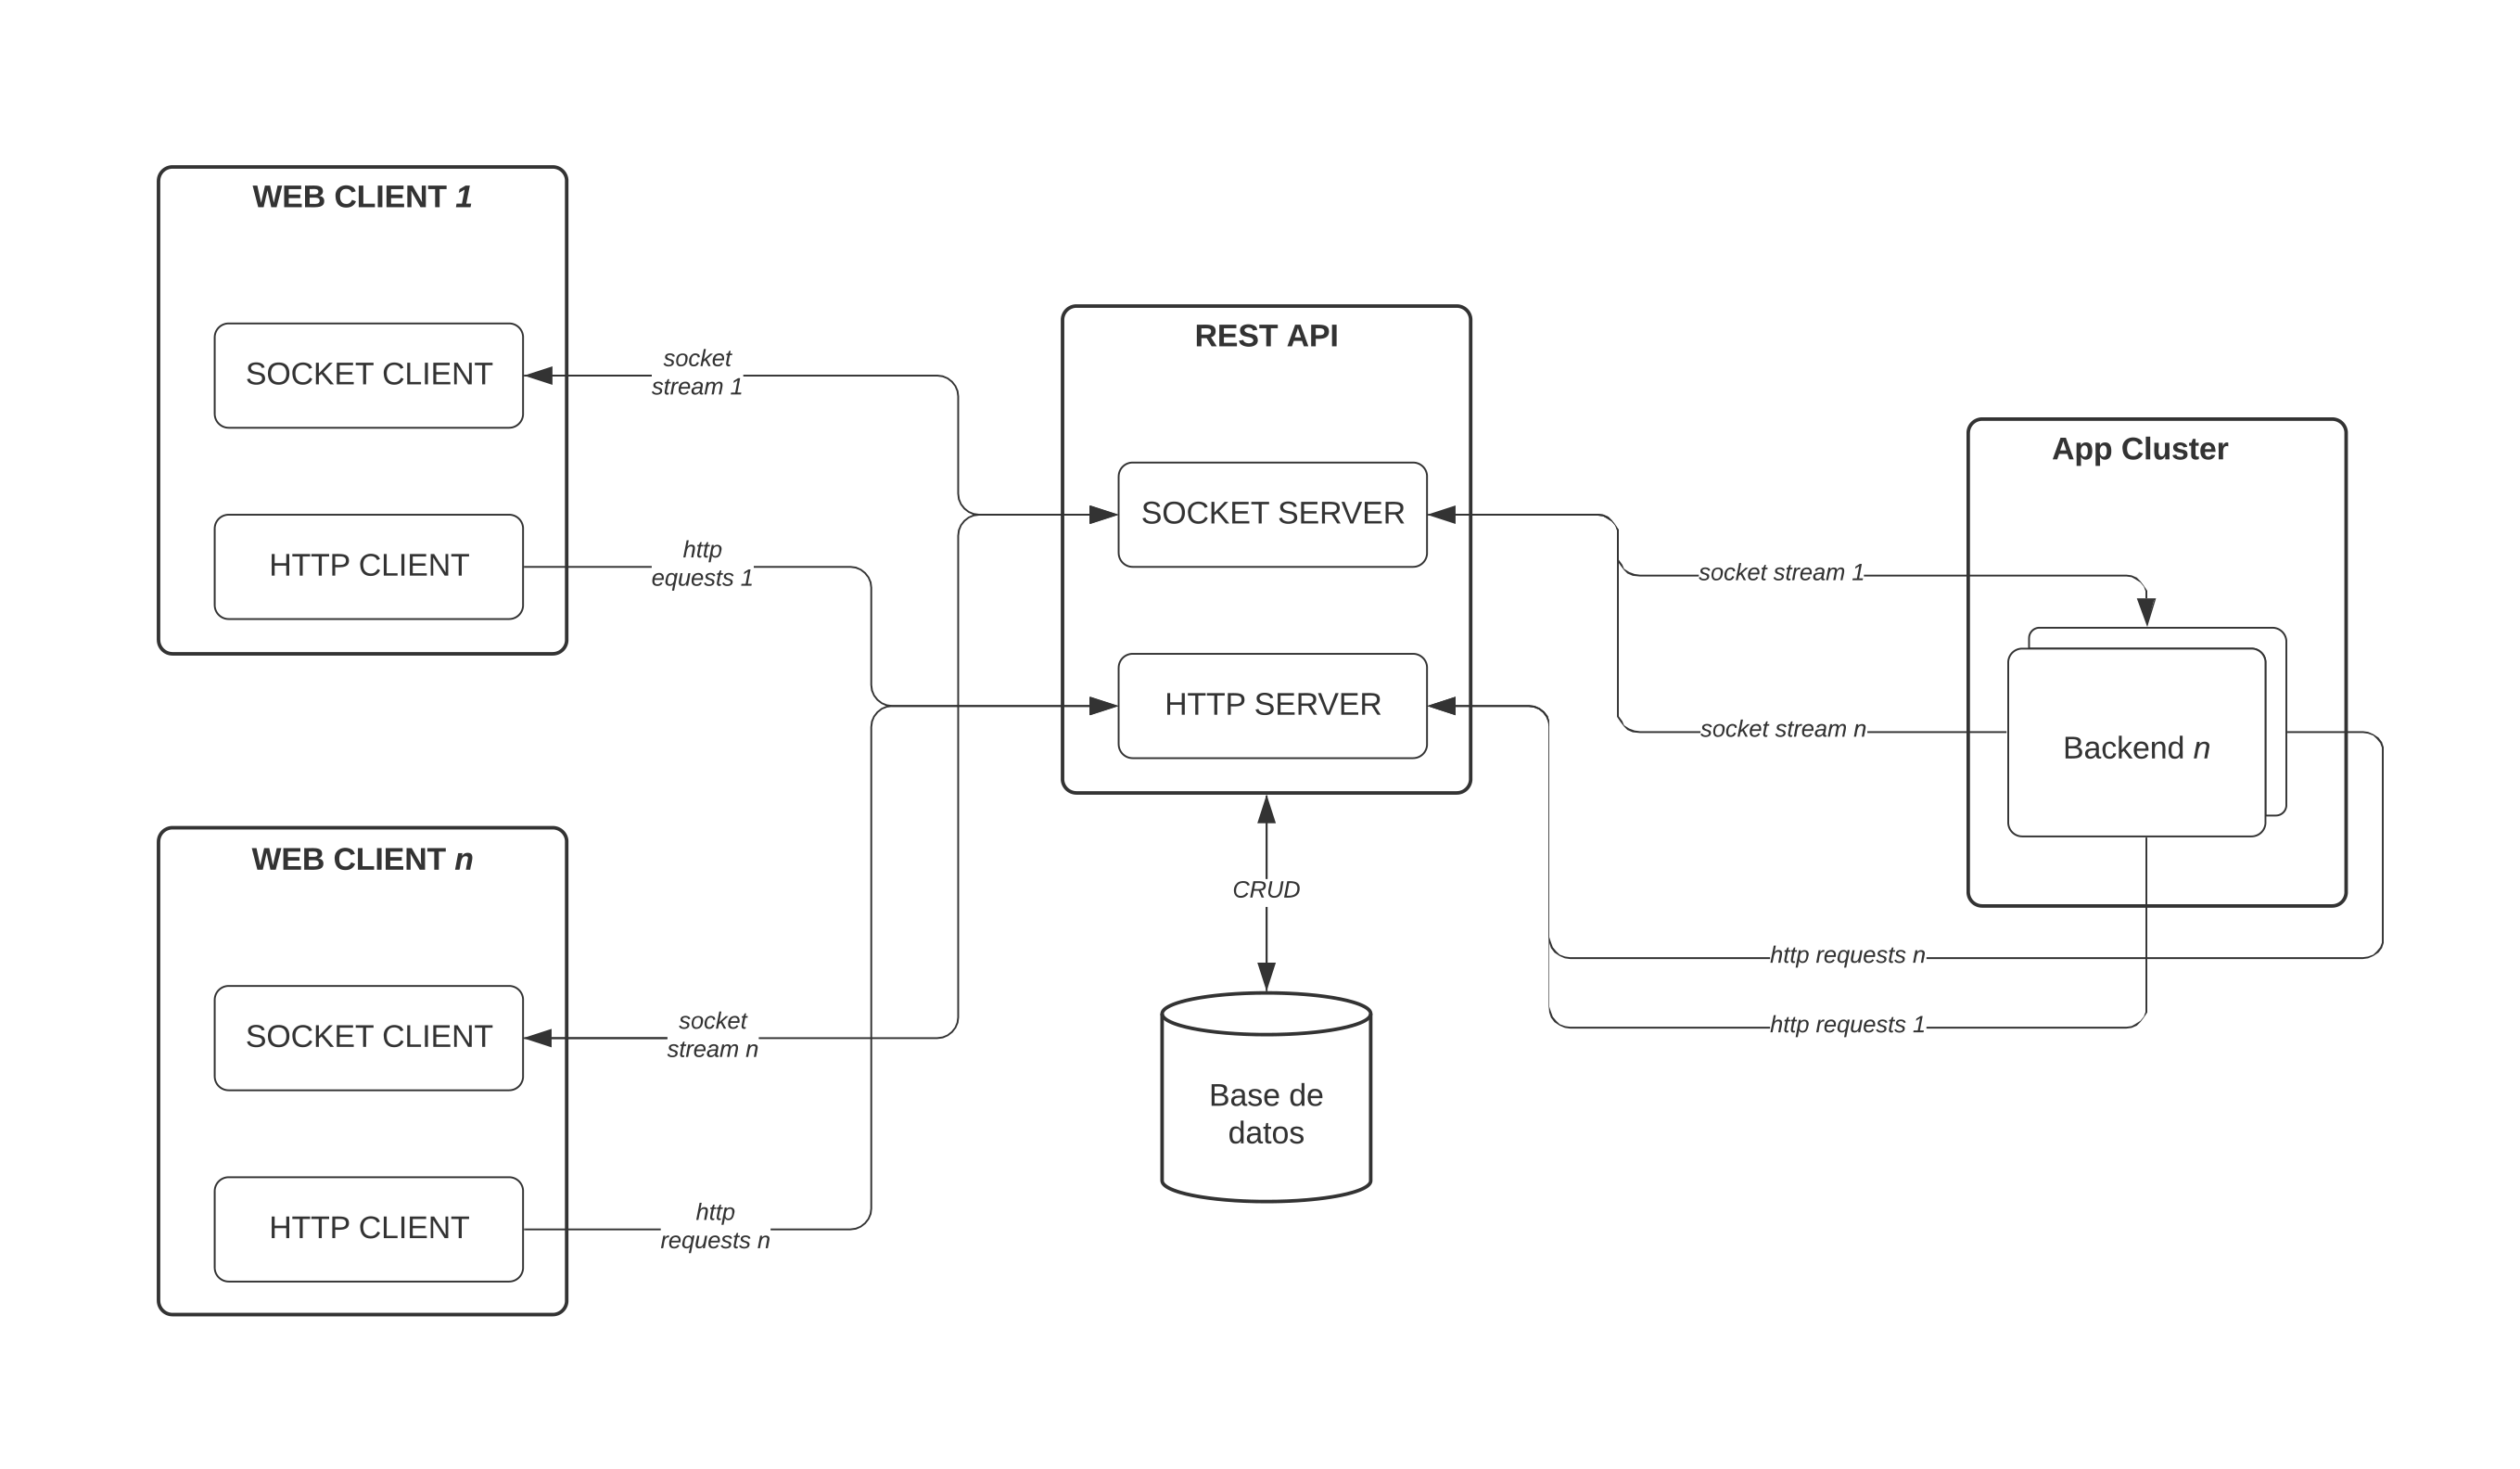
\includegraphics[scale=0.55]{seddi_diagram}}
    \caption{Esquema comunicaciones de servicios en Seddi.}
    \vspace{1.5cm}
  \end{figure}

  En el caso de Author, se trata de una aplicacion web, que utiliza React para la interfaz de usuario, la API de
  Canvas de HTML para el editor 2D y Three.js como motor de render para el editor de 3D. Las interacciones de
  usuario actualizan el estado local del cliente y se comunica con el API REST para persistir los cambios sobre
  los recursos en base de datos. Este flujo permite el disenho y prototipado de la prenda completamente en el
  cliente web, mientras que para las acciones mas costosas, como la simulaci\'on o renderizado offline de tejidos,
  se reserva al usuario un servidor que utiliza un servicio HPC de Seddi encarga de recibir, procesar y enviar la
  peticion a traves del sistema de cola de mensajes.


  \begin{figure}[H]
    \vspace{1cm}
    \centering
      \frame{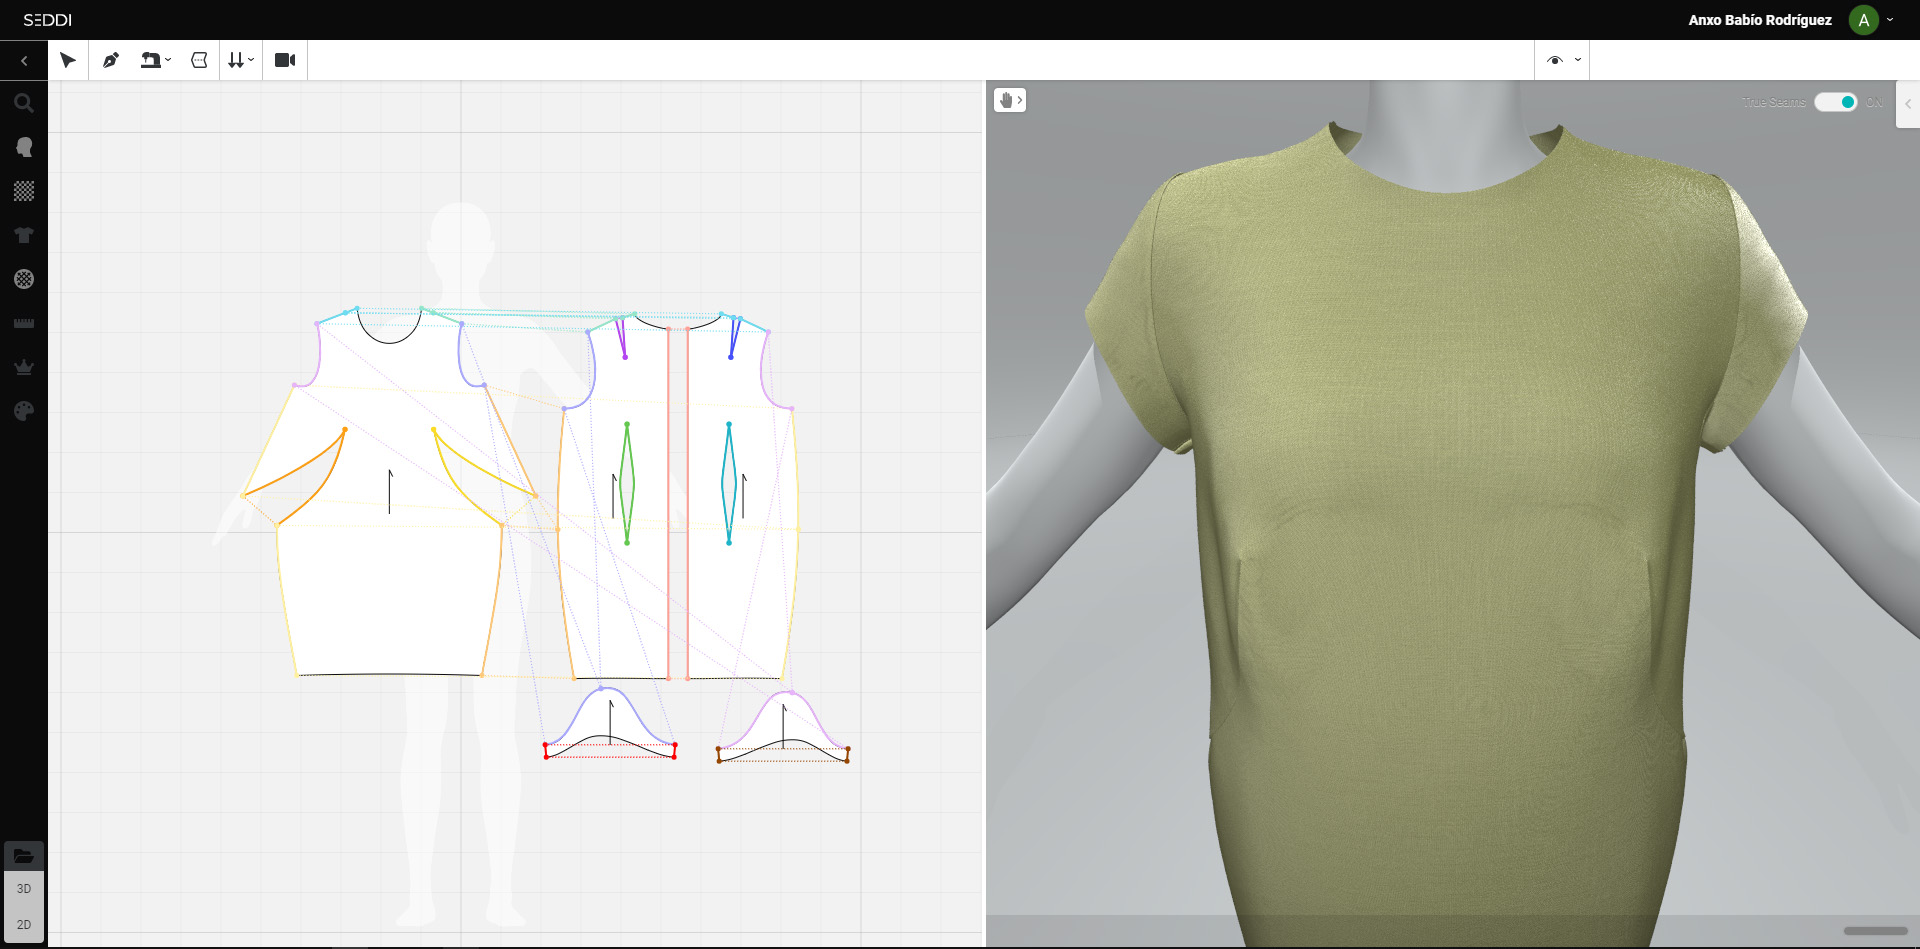
\includegraphics[scale=0.28]{viewports}}
    \caption{Editor de patrones 2D y editor 3D de Author}
    \vspace{0.5cm}
  \end{figure}

  La informacion de un material para que los motores graficos del cliente web y el servicio HPC se almacena en un
  TextureStack, que son resultado de la captura optica de un tejido, o un SurfaceMaterial, la definicion para
  cualquier otro elemento de la escena 3D. Ambos motores graficos utilizan un Entity Component System, por lo que
  la informacion sobre los materiales son una referencia un GarmentPieceComponent, en el caso de un TextureStack,
  o un MeshRenderableComponent, en el caso de un SurfaceMaterial.\\

  Los recursos almacenan diferentes tipos de metadatos, que pueden utilizar diferentes modelos de shading, pero
  comparten la parametrizacion de los materiales. En la figura 4.3 se muestran los esquemas de estos recursos en la
  base de datos.

  \begin{figure}[H]
    \vspace{0.5cm}
    \centering
      \frame{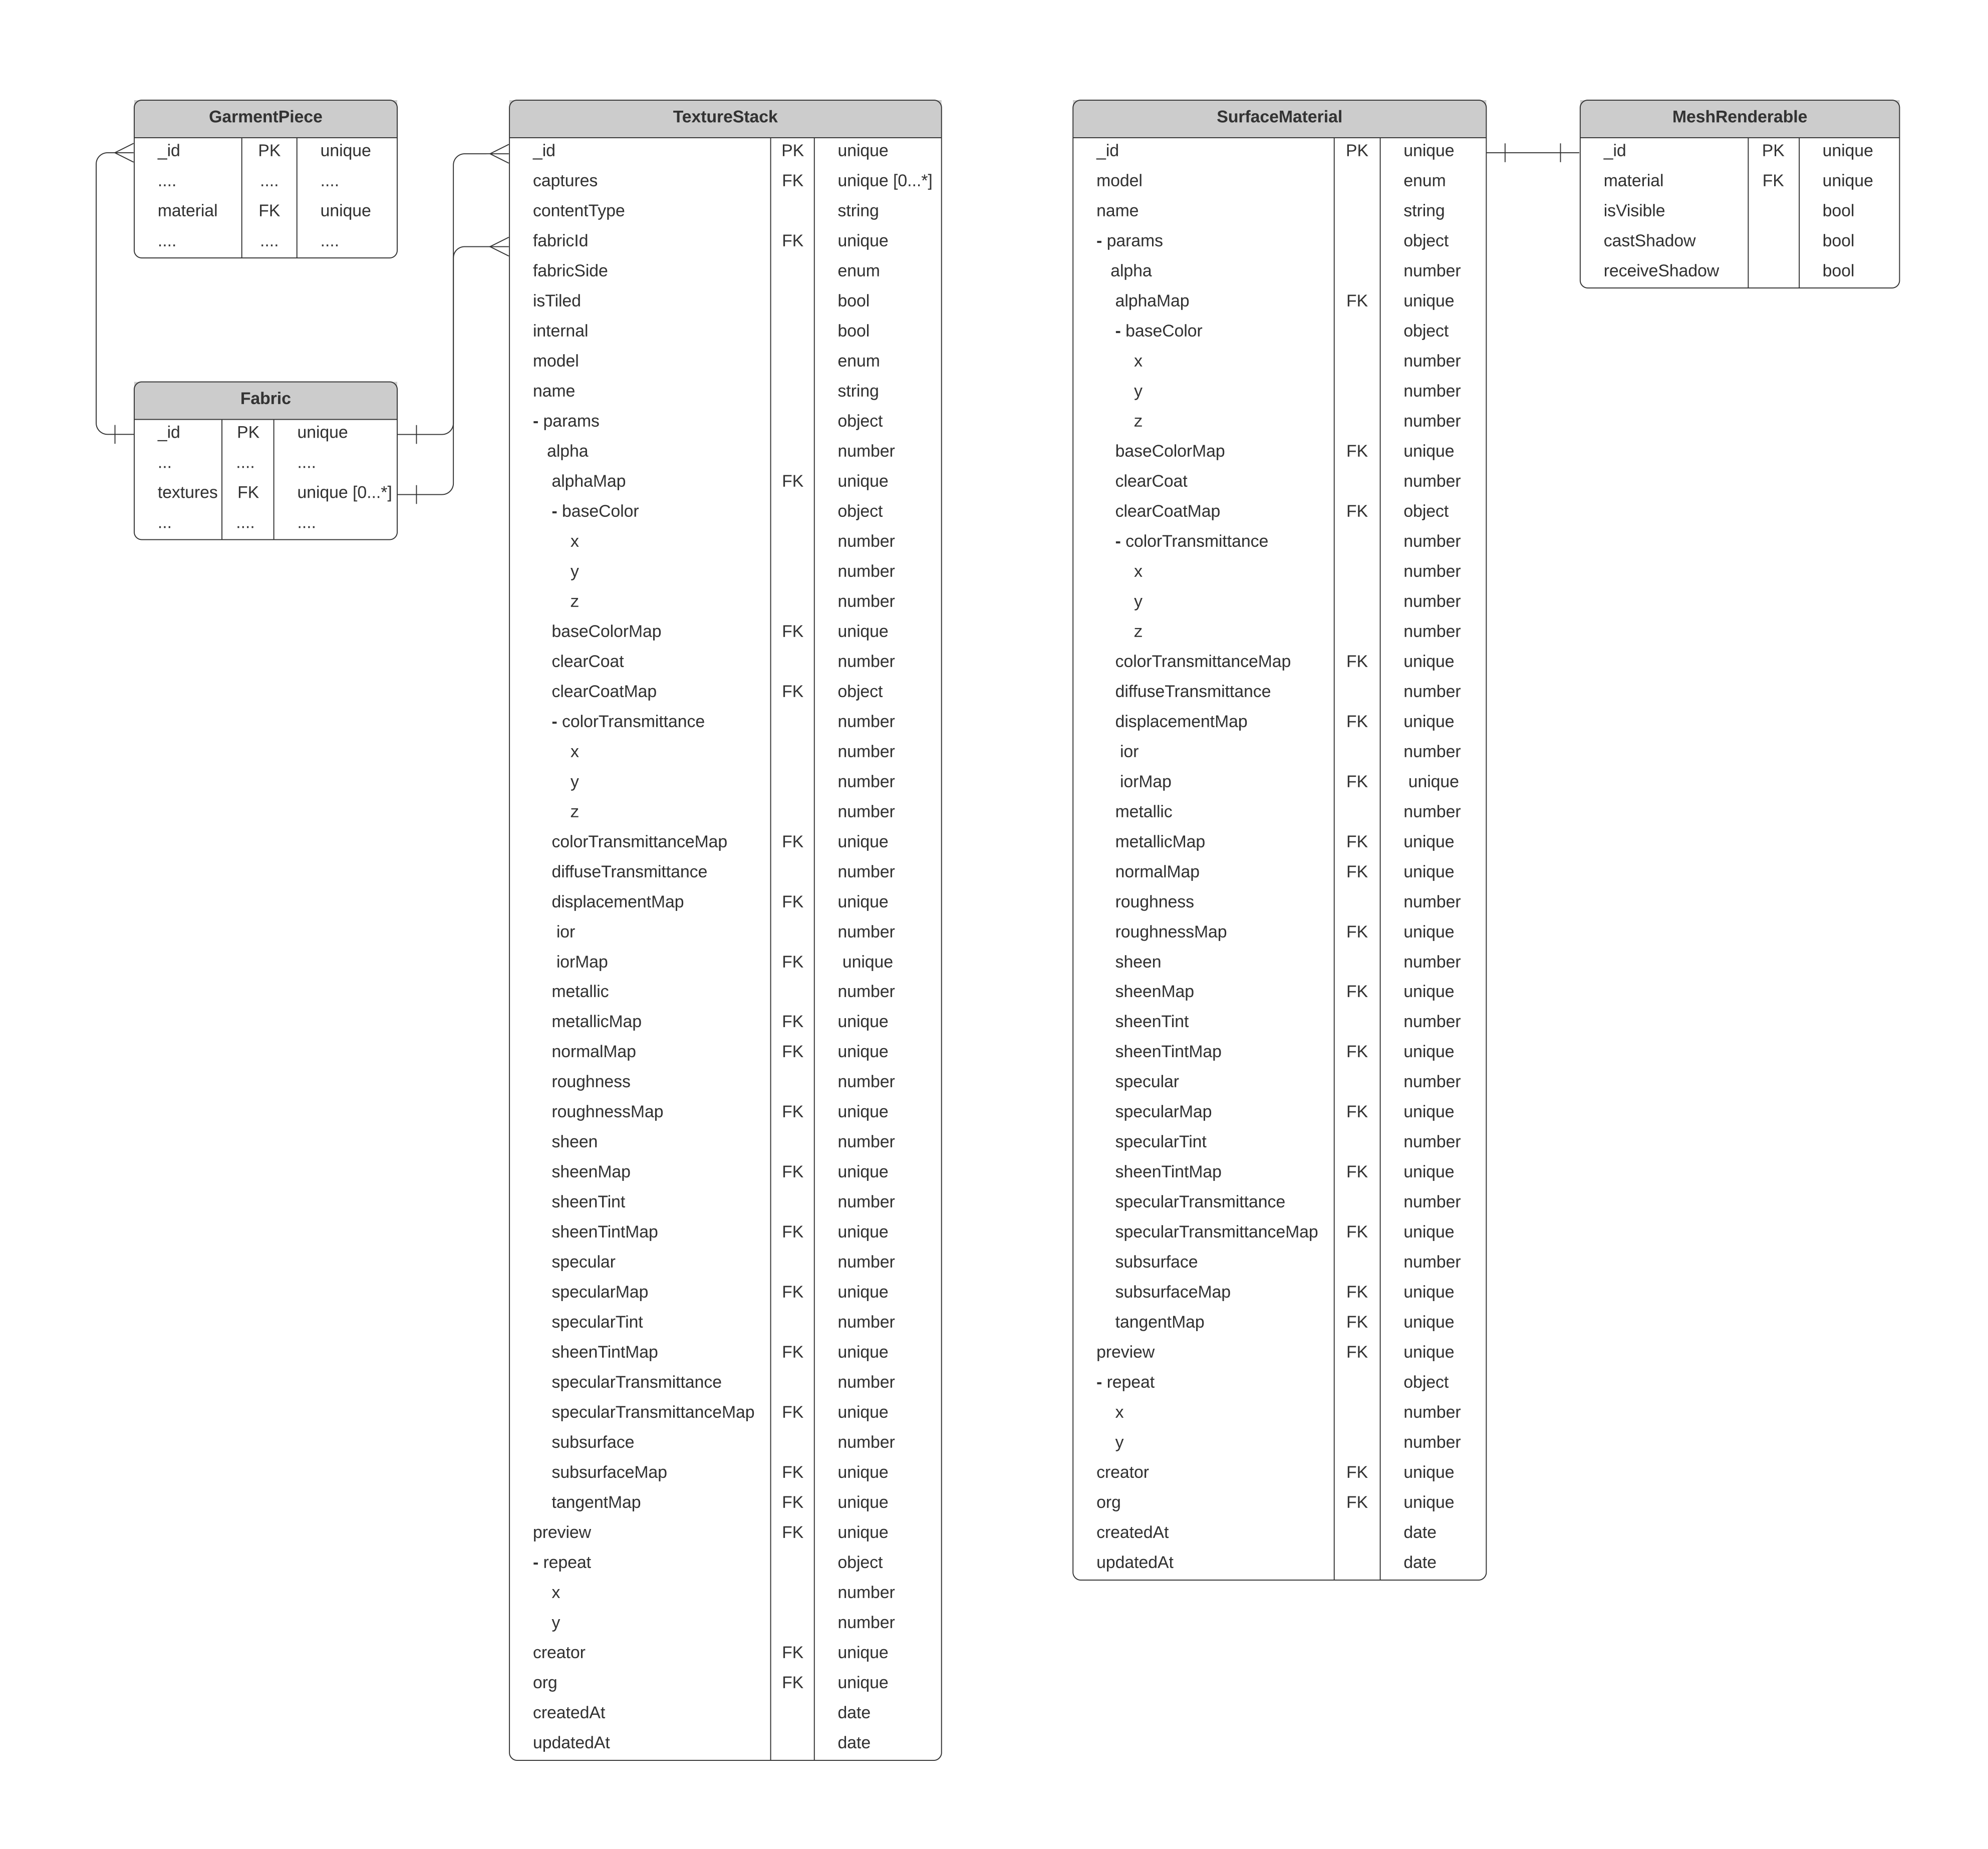
\includegraphics[scale=0.4]{materials_schema}}
    \caption{Modelo de datos de los recursos que utilizan materiales.}
    \vspace{1cm}
  \end{figure}

  El API REST es la interfaz que expone las operaciones disponible sobre este recurso y se documentan con Swagger,
  una herramienta que permite generar documentacion y sirve de guia a los desarrolladores consumidores del API. En
  la figura 4.4 se muestran la documentacion sobre los tipos de peticiones y las rutas del API referidas a recursos
  SurfaceMaterial y TextureStack.

  \begin{figure}[H]
    \vspace{1cm}
    \centering
      \frame{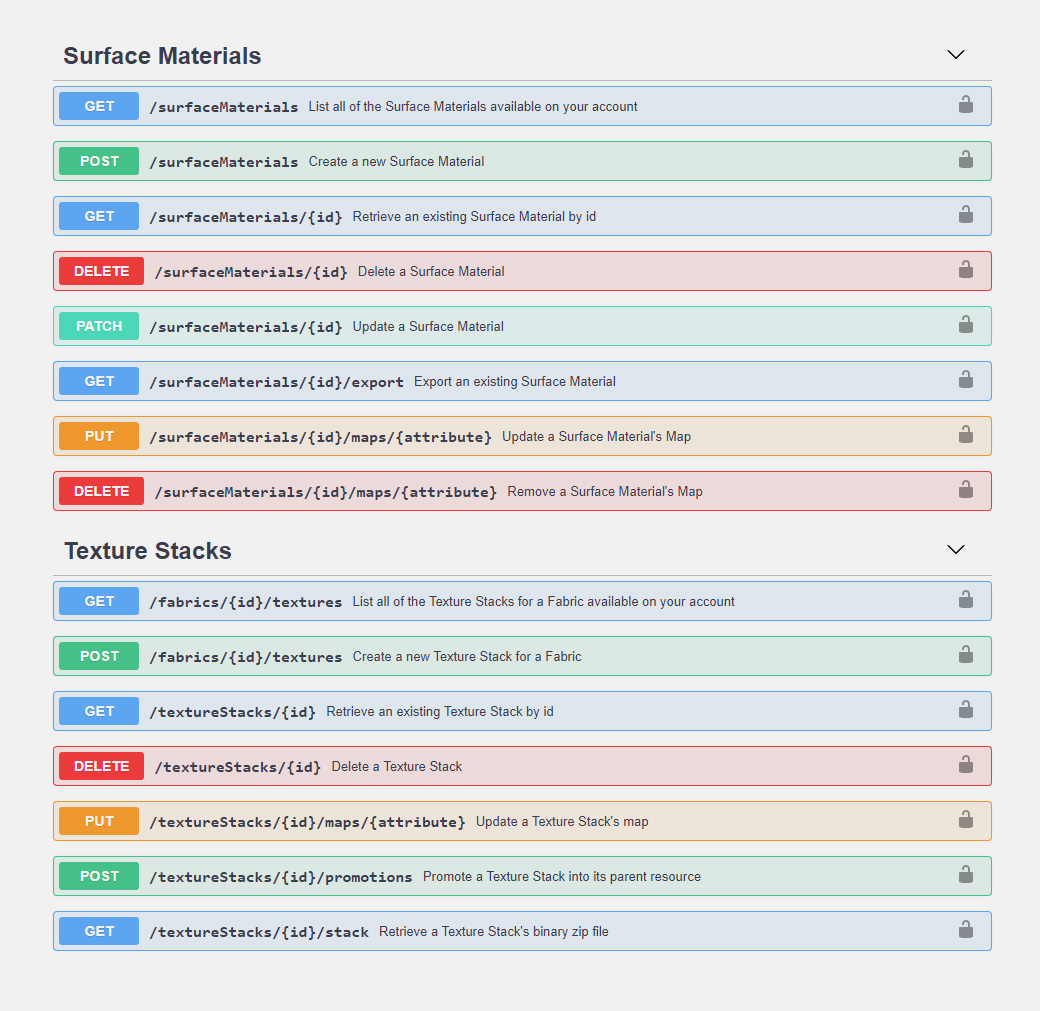
\includegraphics[scale=0.4]{swagger}}
    \caption{Documentaci\'on de los recursos SurafaceMaterial y TextureStack en Swagger.}
    \vspace{1cm}
  \end{figure}
      \chapter{Desarrollo}

\section{Integraci\'on con ThreeJs}
La soluci\'on elegida para extender el sistema de materiales de Three ha sido crear un fork, extendiendo la
librer\'ia para implementar las funcionalidades necesarias que dan soporte a estos nuevos motores de shading.
Siguiendo la nomenclatura, de ThreeJs (MeshStandardMaterial, MeshPhysicalMaeterial, etc) se ha creado un material
MeshClothMaterial, basado en los material Cloth de Filament.\\
ThreeJS utiliza un sistema de chunks (trozos) se componen en tiempo de ejecuci\'on para acabar formando los vertex
y fragment shaders que se utilizan en los programas de WebGL. Los chunks se componen en la libreria de shaders, la
clase ShaderLib.
Para crear nuestro MeshClothMaterial, hemos de extender de la clase base Material, de la que extienden el resto de
materiales. En este caso, de la misma forma que hace MeshPhysicalMaterial, extenderemos de MeshStandardMaterial,
que dispone de la mayor parte de uniforms y attributes que necesita nuestro shader.\\

\bgroup
  \begin{lstlisting}[caption=Clase MeshClothMaterial]
    import { Vector2 } from '../math/Vector2.js';
    import { MeshStandardMaterial } from './MeshStandardMaterial.js';
    import { Color } from '../math/Color.js';
    import brdfCloth from './clothBRDF.js';
    
    /**
     * parameters = {
     *  reflectivity: <float>,
     *
     *  sheen: <Color>,
     *
     *  transmission: <float>,
     *  transmissionMap: new THREE.Texture( <Image> ),
     *
     *  subsurface: <Vector3>,
     * }
     */
    
    function MeshClothMaterial( parameters ) {
    
      MeshStandardMaterial.call( this );
    
      this.defines = {
    
        'STANDARD': '',
        'CLOTH': ''
    
      };
    
      this.type = 'MeshClothMaterial';
      this.sheen = null;
    
      this.transmission = 0.0;
      this.transmissionMap = null;
      this.subsurface = null;
    
      this.brdfCloth = brdfCloth;
    
      this.setValues( parameters );
    
    }
    
    MeshClothMaterial.prototype = Object.create( MeshStandardMaterial.prototype );
    MeshClothMaterial.prototype.constructor = MeshClothMaterial;
    
    MeshClothMaterial.prototype.isMeshClothMaterial = true;
    
    MeshClothMaterial.prototype.copy = function ( source ) {
    
      MeshStandardMaterial.prototype.copy.call( this, source );
    
      this.defines = {
    
        'STANDARD': '',
        'CLOTH': ''
    
      };
    
      if ( source.sheen ) {
    
        this.sheen = ( this.sheen || new Color() ).copy( source.sheen );
    
      }
    
      this.transmission = source.transmission;
      this.transmissionMap = source.transmissionMap;
    
      if ( source.subsurface ) {
    
        this.subsurface = ( this.subsurface || new Color() ).copy( source.subsurface );
    
      } else {
    
        this.subsurface = null;
    
      }
    
      if ( source.brdfCloth ) {
    
        this.brdfCloth = source.brdfCloth;
    
      } else {
    
        this.brdfCloth = null;
    
      }
    
      return this;
    
    };
    
    export { MeshClothMaterial };
    
  \end{lstlisting}
  
  Para que el motor de render de ThreeJS reconozca este nuevo material es necesario, a\~nadir
  su tipo (MeshClothMaterial) al mapa de ShaderIds para que el gestor de programas (WebGLPrograms)
  lo utilice para detectar obtener los uniforms y shaders necesarios para el material. Adem\'as
  los nuevos par\'ametros necesarios para el material se deben de incluir en el array
  parametersNames, de forma que el sistema de cacheo de programas de ThreeJS detecte estas
  nuevas propiedades.\newline
  
  \begin{lstlisting}[caption=Clase MeshClothMaterial]
  function WebGLPrograms( renderer, cubemaps, extensions, capabilities, bindingStates, clipping ) {
  
    // ...
  
    const shaderIDs = {
      MeshDepthMaterial: 'depth',
      MeshDistanceMaterial: 'distanceRGBA',
      MeshNormalMaterial: 'normal',
      MeshBasicMaterial: 'basic',
      MeshLambertMaterial: 'lambert',
      MeshPhongMaterial: 'phong',
      MeshToonMaterial: 'toon',
      MeshStandardMaterial: 'physical',
      MeshPhysicalMaterial: 'physical',
      MeshClothMaterial: 'cloth',
      MeshMatcapMaterial: 'matcap',
      LineBasicMaterial: 'basic',
      LineDashedMaterial: 'dashed',
      PointsMaterial: 'points',
      ShadowMaterial: 'shadow',
      SpriteMaterial: 'sprite'
    };
  
    const parameterNames = [
      "precision", "isWebGL2", "supportsVertexTextures", "outputEncoding", "instancing", "instancingColor",
      "map", "mapEncoding", "matcap", "matcapEncoding", "envMap", "envMapMode", "envMapEncoding", "envMapCubeUV",
      "lightMap", "lightMapEncoding", "aoMap", "emissiveMap", "emissiveMapEncoding", "bumpMap", "normalMap", "objectSpaceNormalMap", "tangentSpaceNormalMap", "clearcoatMap", "clearcoatRoughnessMap", "clearcoatNormalMap", "displacementMap", "specularMap", "subsurface", "brdfCloth",
      "roughnessMap", "metalnessMap", "gradientMap",
      "alphaMap", "combine", "vertexColors", "vertexTangents", "vertexUvs", "uvsVertexOnly", "fog", "useFog", "fogExp2",
      "flatShading", "sizeAttenuation", "logarithmicDepthBuffer", "skinning",
      "maxBones", "useVertexTexture", "morphTargets", "morphNormals",
      "maxMorphTargets", "maxMorphNormals", "premultipliedAlpha",
      "numDirLights", "numPointLights", "numSpotLights", "numHemiLights", "numRectAreaLights",
      "numDirLightShadows", "numPointLightShadows", "numSpotLightShadows",
      "shadowMapEnabled", "shadowMapType", "toneMapping", 'physicallyCorrectLights',
      "alphaTest", "doubleSided", "flipSided", "numClippingPlanes", "numClipIntersection", "depthPacking", "dithering",
      "sheen", "transmissionMap"
    ];
  
    // ...
  
    function getParameters( material, lights, shadows, scene, object ) {
  
      const shaderID = shaderIDs[ material.type ];
  
      // ...
  
      let vertexShader, fragmentShader;
  
      if ( shaderID ) {
  
        const shader = ShaderLib[ shaderID ];
  
        vertexShader = shader.vertexShader;
        fragmentShader = shader.fragmentShader;
  
      }
  
      // ...
  
      const parameters = {
  
        shaderID: shaderID,
  
        vertexShader: vertexShader,
        fragmentShader: fragmentShader,
  
        sheen: !! material.sheen,
  
        subsurface: !! material.subsurface,
  
        brdfCloth: !! envMap && shaderID === 'MeshClothMaterial',
        // ...
      };
  
      // ...
  
      return parameters;
    }
  \end{lstlisting}
  
  Finalmente, en el gestor de materiales de ThreeJs, necesitamos a\~nadir un nuevo m\'etodo
  que actualice los unfiroms del programa creado, de la misma forma que se hace con los
  materiales nativos de la librer\'ia.\newline
  
  \begin{lstlisting}[caption=Clase WebGLMaterials]
  function refreshMaterialUniforms( uniforms, material, pixelRatio, height ) {
  
  // ...
  
  if ( material.isMeshStandardMaterial ) {
  
    refreshUniformsCommon( uniforms, material );
  
    if ( material.isMeshPhysicalMaterial ) {
  
      refreshUniformsPhysical( uniforms, material );
  
    } else if ( material.isMeshClothMaterial ) {
  
      refreshUniformsCloth( uniforms, material );
  
    } else {
  
      refreshUniformsStandard( uniforms, material );
  
    }
  
  }
  
  // ...
  
  function refreshUniformsCloth( uniforms, material, environment ) {
  
    refreshUniformsStandard( uniforms, material, environment );
  
    uniforms.reflectivity.value = material.reflectivity; // also part of uniforms common
  
    if ( material.sheen ) {
  
      uniforms.sheen.value.copy( material.sheen );
  
    } else {
  
      uniforms.sheen.value.copy( material.color );
      uniforms.sheen.value.r = Math.sqrt( uniforms.sheen.value.r );
      uniforms.sheen.value.g = Math.sqrt( uniforms.sheen.value.g );
      uniforms.sheen.value.b = Math.sqrt( uniforms.sheen.value.b );
  
    }
  
    if ( material.subsurface ) uniforms.subsurface.value.copy( material.subsurface );
  
    if ( material.brdfCloth ) uniforms.brdfCloth.value = material.brdfCloth;
  
  }
    
  \end{lstlisting}
  
  De esta forma, tenemos un material con la interfaz nativa de ThreeJS, que tiene acceso a los
  chunks definidos en la clase ShaderChunk y cuyos uniforms y composici\'on de chunks definiremos
  en ShaderLib.\newline
  
  El BRDF para el componente especular de la iluminaci\'on directa del material Cloth de Filament,
  se utiliza en ThreeJS para a\~nadir opcionalmente un l\'obulo de Sheen al material. Por otra
  parte, el difuso, utiliza en Filament un t\'ermino opcional para ofrecer una aproximaci\'on
  barata el subsurface scattering para iluminaci\'on directa que utiliza Filament.\newline
  
  \begin{lstlisting}[caption=Implementaci\'on del BRDF de iluminaci\'on directa de Filament]
    vec3 surfaceShading(const PixelParams pixel, const Light light) {
      vec3 h = normalize(shading_view + light.l);
      float NoL = light.NoL;
      float NoH = saturate(dot(shading_normal, h));
      float LoH = saturate(dot(light.l, h));
  
      // specular BRDF
      float D = D_Charlie(pixel.roughness, NoH);
      float V = V_Neubelt(shading_NoV, NoL);
      vec3  F = pixel.f0; // f0 is sheen color for Cloth materials 
      vec3 Fr = (D * V) * F;
  
      // diffuse BRDF
      float diffuse = diffuse(pixel.roughness, shading_NoV, NoL, LoH);
      #if defined(MATERIAL_HAS_SUBSURFACE_COLOR)
        diffuse *= Fd_Wrap(dot(shading_normal, light.l), 0.5);
      #endif
  
      vec3 Fd = diffuse * pixel.diffuseColor;
  
    #if defined(MATERIAL_HAS_SUBSURFACE_COLOR)
      Fd *= saturate(pixel.subsurfaceColor + NoL);
      vec3 color = ( Fd + Fr * NoL ) * light.colorIntensity
    #else
      vec3 color = Fd + Fr * NoL * light.colorIntensity;
    #endif
  
    return color;
  }
  \end{lstlisting}
  
  Primero definimos la interfaz de nuestro MeshClothMaterial y pondremos en comparaci\'on con
  el MeshPhysicalMaeterial, para analizar los par\'ametros en com\'un y los cambios en sus BRDF
  y ecuaciones de render.\newline
  
  \centering
  \begin{tabular}{| c | c |}
    \hline
    MeshPhysicalMaterial & MeshClothMaterial \\ \hline
    color & color \\
    roughness & roughness \\
    clearCoat & NO \\
    clearCoatRoughness & NO \\
    sheen  & sheen  \\
    NO  & subsurface  \\
    metalness & NO \\
    emissive & emissive \\
    alpha & alpha \\
    lightmap & lightmap \\
    normalMap & normalMap \\ \hline
  \end{tabular}\\
\egroup


\section{BRDF}
El MeshPhysicalMaeterial usa GGX, \autocite{ggx}.
Al contrario que el MeshPhysicalMaterial, que utiliza una una distribucion GGX, el material
Cloth de Filament utiliza una  version modificada del BRDF presentado por Ashikmin y Premoze
\autocite{velvet}

$$
D_{Velvet}(v, h, \alpha) = c_{norm} (
	1 + 4exp \left(\frac{-cot^2\theta_h}{\alpha^2}\right)
)
$$

en su lugar se utiliza la la presentada por Est\'evez y Kulla \autocite{sheen}

$$
  D_{Charlie}(\alpha) = \frac
    {(2 + \frac{1}{\alpha})sin(\theta)^\frac{1}{\alpha}}
    {2\pi}
$$

y se utiliza una version modificada del denominador para suavizar:

$$
\frac{1}{4(N\cdot{V})(N\cdot{L})}
$$

Por su parte, el difuso, aunque muy parecido al de Threejs, que utiliza un BRDF de Lambert,
Filmament anhade un factor de correccion que permite simular el efecto de subsurface.

$$
f_d(v, h) = \frac{c_{diff}}{\pi}(1 - F(v, h))
\Bigg\langle
n\cdot{l} + \frac{w}{(1+ w)^2}\langle c_{subsurface} + n \cdot{l} \rangle
\Bigg\rangle
$$

\section{Iluminaci\'on indirecta}
Para los efectos de iluminacion global, se necesita conocer la irradiancia proviniente en todas
direcciones $w_i$ sobre la esfera $\Omega$.

\begin{figure}[H]
  \vspace{0.5cm}
  \centering
    \frame{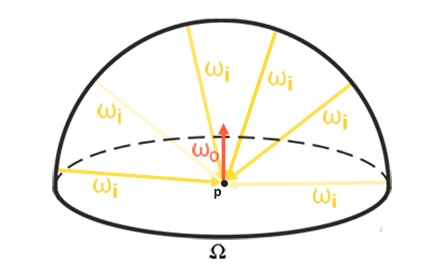
\includegraphics[scale=0.5]{hemisphere}}
  \caption{hemisphere}
\end{figure}

La ecuacion de render describe la radiancia de salida sobre un punto.
$$
L_o(p, w_o) = \int_{\Omega} f_r(p, w_i, w_o)L_i(p, w_i)n\cdot{w_i}dw_i
$$

Siendo $\Omega$ la hemiesfera centrada en el punto sobre la que calculamos la irradiancia,
$f_r$ representa el brdf, $Li$, la irradiancia de la escena, mientras que $n\cdot{w_i}$ toma en
cuenta el \'angulo entre la de incidencia de la luz sobre la superficie.

$$
L_o(p, w_o) = \int_{\Omega} (k_d + \frac{c}{\pi} + 
k_s \frac{DFG}{4(w_o\cdot{n})(w_i\cdot{n})})L_i(p, w_i)n\cdot{w_i}dw_i
$$

Los terminos $k_s$ y $k_d$ de la ecuacion de reflectancia son independientes, por lo que, de la
misma forma que en la iluminacion directa, los componentes se pueden separar en difuso y
especular.

$$
L_o(p, w_o) = \int_{\Omega}
(k_d \frac{c}{\pi}) L_i(p, w_i)n\cdot{w_i}dw_i +
\int_{\Omega} 
k_s \frac{DFG}{4(w_o\cdot{n})(w_i\cdot{n})})L_i(p, w_i)n\cdot{w_i}dw_i
$$

La soluci\'on de la integral de la irradiancia de salida sobre $\Omega$ requiere samplear el entorno
en todas las direcciones posibles. Es por ello que en tiempo real, la soluci\'on consiste en
precomputar este c\'alculo y durante la ejecucion, calcular esta tabla de resultados.\\
ThreeJs utiliza dos enfoques, por una parte, mapas de irradiancia y por otra, light probes, que
utilizan spherical harmonics. Los mapas de irradiancia son una tecnica IBL (Image Based Lighting)
tratan todo el entorno como una fuente de luz y utilizan im\'agenes precomputadas que permiten
acelerar este calculo. Estas t\'ecnicas, aunque muy eficientes durante la ejecucion, son muy
costosas como para generarlas en tiempo real bajo demanda, la tecnica spherical harmonics, una
t\'ecnica que reduce el coste de generacion de los mapas de entorno a costa de comprimir la
informacion de irradiancia en un representacion frecuencias frente a espacio.

\subsection{Componente especular}
Para el especular, la tanto ThreeJs utilizan la t\'ecnica split-sum approximation
\autocite{splitsum}. \'Esta t\'ecnica permite separar la en dos partes la soluci\'on de la
integral.

$$
L_o(p, w_o) =
\int_{\Omega} 
  k_s \frac{DFG}{4(w_o\cdot{n})(w_i\cdot{n})})L_i(p, w_i)n\cdot{w_i}dw_i =
\int_{\Omega} k_s \frac{DFG}{4(w_o\cdot{n})(w_i\cdot{n})}) *
\int_{\Omega}L_i(p, w_i)n\cdot{w_i}dw_i
$$

Por una parte, el mapa prefiltrado de entorno es un mapa preconvolucionado que tiene en cuenta
los posibles valores de rugosidad del material de forma que a medida que el ruido es mayor, las
reflexiones son de un color menos definido. Esta tecnica utiliza simplifica el calculo de
la integral asumiendo la direccion de la vista igual a la direccion de sampleo.\\
Por otra parte, el c\'alculo del BRDF se almacena en una textura, conocida como mapa de integral
del BRDF, utilizando $n\cdot{w_i}$ en el eje $x$ y $roughness$ en el eje y.

\begin{figure}[H]
  \vspace{0.5cm}
  \centering
    \frame{
\includegraphics[scale=0.5]{dfg_cloth}}
  \caption{DFG cloth}
  \vspace{0.5cm}
\end{figure}

ThreeJs utiliza la aproximaci\'on anal\'itica para el c\'alculo de de mapa de integral del BRDF,
la presentada por Epic Garmes \autocite{shadingmobile}, para aproximar el c\'alculo el BRDF GGX.

\begin{lstlisting}[caption=Apromixaci\'on anal\'itica a la integral del BRDF en ThreeJs]
vec2 integrateSpecularBRDF( const in float dotNV, const in float roughness ) {
  const vec4 c0 = vec4( - 1, - 0.0275, - 0.572, 0.022 );
  const vec4 c1 = vec4( 1, 0.0425, 1.04, - 0.04 );
  vec4 r = roughness * c0 + c1;
  float a004 = min( r.x * r.x, exp2( - 9.28 * dotNV ) ) * r.x + r.y;
  return vec2( -1.04, 1.04 ) * a004 + r.zw;
}
\end{lstlisting}

Sin embargo, \'este c\'aculo no es v\'alido para nuestro BRDF, por que, deberemos utilizar una
tabla en la que almacenar los resultados calculados para el BRDF presentado por Est\'evez y Kulla.


\subsection{Componente difusa}
      \chapter{Resultados}
    \appendix
      \addcontentsline{toc}{chapter}{Appendix}
      \chapter{Conceptos b\'asicos}

\section{Unidades b\'asicas radiom\'etricas}
\todo[inline]{Cambiar/completar}

\bgroup
    Cuando hablamos de la cantidad de luz, no es la medicion sobre un foton de luz independiente, si no que se tratan de medidas en relacion
    al tiempo, la direccion o el \'area.

    \begin{itemize}
    \item[] \textbf {{\'Angulo s\'olido}}
    \item[] \textbf {Flujo} La unidad que representa la energia sobre la unidad de tiempo es el flujo, representado por Phi. Es la energía que transportan las ondas
    por unidad de tiempo, se mide en vatios. En los motores de render se utiliza para expresar la cantidad total de energia emitida por un a fuente de luz.
    \begin{equation}
        \Phi_e = \dfrac{d{Q_e}}{dt}
    \end{equation}
    \item[] \textbf {Intensidad}
    \begin{equation}
        I = \dfrac{d\Phi}{d\omega}
    \end{equation} 
    \item[] \textbf {Irradiancia} La irradiancia, es la cantidad de energ\'ia por unidad de tiempo por unidad de superficie, o flujo por superficie. Se representa como
    E, su unidad son los vatios/m2 y se utiliza para medir la cantidad de luz que incide sobre una superficie.
    \begin{equation}
        E = \dfrac{d\Phi}{dA}
    \end{equation}
    Cuando este flujo de radiancia se mide en direcci\'on contraria, de salida, se llama emitancia (M)
    \item[] \textbf {Radiancia} Simula luz tan lejana que sus rayos son paralelos entre si, como por ejemplo el sol.
    \begin{equation}
        L = \dfrac{d^2\Phi}{dA_{proj}d\omega}
    \end{equation}
    \end{itemize}
\egroup

\section{BxDF}
    \bgroup
    A continuaci\'on se detallan los nombres de las funciones en funcion del fen\'omeno f\'isico que modelan.
    \begin{itemize}
        \item[] \textbf {BRDF} Es la funci\'on que modela el comportamiento de la luz al golpear una superficie opaca, la reflexi\'on. Fue definido por primera vez en 1965 por
        Fred Nicodemus y su definici\'on es el ratio entre radiancia reflectada e irraciancia incidente.
        Para determinar el \'angulo de salida del rayo se utiliza la ley de la reflexi\'on y las tres caracter\'isticas que ha de cumplir un BRDF basado en
        f\'isica es que sea positivo, que cumpla con la reciprocidad de Helmholtz y que cumpla con la ley de conservaci\'on de la energ\'ia.
        \item[] \textbf {BTDF} Describe el comportamiento del rayo de luz al atravesar una superficie, la refracci\'on. Para calcular el angulo de salida del rayo se utiliza la
        ley de Snell, y al contrario que el BRDF, no sumple el principio de reciprocidad de Helmholtz.
        \item[] \textbf {BSSRDF y BSSTF} Son ampliaciones del modelo de reflexi\'on y refracci\'on, respectivamente, teniendo en cuenta las reflexiones internas del rayo a traves de la
        superficie del objeto.
        \item[] \textbf {BSDF} Se utiliza comunmente para hablar de cualquier forma de BxDF. En un sentido mas estricto, se refiere al conjunto de un BSSRDF y un BSSTDF.
    \end{itemize}
    \egroup

    \section{Integraci\'on con ThreeJs}
    La soluci\'on elegida para extender el sistema de materiales de Three ha sido crear un fork, extendiendo la
    librer\'ia para implementar las funcionalidades necesarias que dan soporte a estos nuevos motores de shading.
    Siguiendo la nomenclatura, de ThreeJs (MeshStandardMaterial, MeshPhysicalMaterial, etc) se ha creado un material
    MeshClothMaterial, basado en los material Cloth de Filament.\\
    ThreeJs utiliza un sistema de chunks (trozos) se componen en tiempo de ejecuci\'on para acabar formando los vertex
    y fragment shaders que se utilizan en los programas de WebGL. Los chunks se componen en la libreria de shaders, la
    clase ShaderLib.
    Para crear nuestro MeshClothMaterial, hemos de extender de la clase base Material, de la que extienden el resto de
    materiales. En este caso, de la misma forma que hace MeshPhysicalMaterial, extenderemos de MeshStandardMaterial,
    que dispone de la mayor parte de uniforms y attributes que necesita nuestro shader.\\

    \bgroup

    \begin{lstlisting}[caption=Clase MeshClothMaterial]
import { Vector2 } from '../math/Vector2.js';
import { MeshStandardMaterial } from './MeshStandardMaterial.js';
import { Color } from '../math/Color.js';
import brdfCloth from './clothBRDF.js';

/**
    * parameters = {
    *  reflectivity: <float>,
    *
    *  sheen: <Color>,
    *
    *  transmission: <float>,
    *  transmissionMap: new THREE.Texture( <Image> ),
    *
    *  subsurface: <Vector3>,
    * }
    */

function MeshClothMaterial( parameters ) {

    MeshStandardMaterial.call( this );

    this.defines = {

    'STANDARD': '',
    'CLOTH': ''

    };

    this.type = 'MeshClothMaterial';
    this.sheen = null;

    this.transmission = 0.0;
    this.transmissionMap = null;
    this.subsurface = null;

    this.brdfCloth = brdfCloth;

    this.setValues( parameters );

}

MeshClothMaterial.prototype = Object.create( MeshStandardMaterial.prototype );
MeshClothMaterial.prototype.constructor = MeshClothMaterial;

MeshClothMaterial.prototype.isMeshClothMaterial = true;

MeshClothMaterial.prototype.copy = function ( source ) {

    MeshStandardMaterial.prototype.copy.call( this, source );

    this.defines = {

    'STANDARD': '',
    'CLOTH': ''

    };

    if ( source.sheen ) {

    this.sheen = ( this.sheen || new Color() ).copy( source.sheen );

    }

    this.transmission = source.transmission;
    this.transmissionMap = source.transmissionMap;

    if ( source.subsurface ) {

    this.subsurface = ( this.subsurface || new Color() ).copy( source.subsurface );

    } else {

    this.subsurface = null;

    }

    if ( source.brdfCloth ) {

    this.brdfCloth = source.brdfCloth;

    } else {

    this.brdfCloth = null;

    }

    return this;

};

export { MeshClothMaterial };
        
    \end{lstlisting}
    
    Para que el motor de render de ThreeJs reconozca este nuevo material es necesario, a\~nadir
    su tipo (MeshClothMaterial) al mapa de ShaderIds para que el gestor de programas (WebGLPrograms)
    lo utilice para detectar obtener los uniforms y shaders necesarios para el material. Adem\'as
    los nuevos par\'ametros necesarios para el material se deben de incluir en el array
    parametersNames, de forma que el sistema de cacheo de programas de ThreeJs detecte estas
    nuevas propiedades.\newline
    
    \begin{lstlisting}[caption=Clase MeshClothMaterial]
function WebGLPrograms( renderer, cubemaps, extensions, capabilities, bindingStates, clipping ) {

// ...

const shaderIDs = {
    MeshDepthMaterial: 'depth',
    MeshDistanceMaterial: 'distanceRGBA',
    MeshNormalMaterial: 'normal',
    MeshBasicMaterial: 'basic',
    MeshLambertMaterial: 'lambert',
    MeshPhongMaterial: 'phong',
    MeshToonMaterial: 'toon',
    MeshStandardMaterial: 'physical',
    MeshPhysicalMaterial: 'physical',
    MeshClothMaterial: 'cloth',
    MeshMatcapMaterial: 'matcap',
    LineBasicMaterial: 'basic',
    LineDashedMaterial: 'dashed',
    PointsMaterial: 'points',
    ShadowMaterial: 'shadow',
    SpriteMaterial: 'sprite'
};

const parameterNames = [
    "precision", "isWebGL2", "supportsVertexTextures", "outputEncoding", "instancing", "instancingColor",
    "map", "mapEncoding", "matcap", "matcapEncoding", "envMap", "envMapMode", "envMapEncoding", "envMapCubeUV",
    "lightMap", "lightMapEncoding", "aoMap", "emissiveMap", "emissiveMapEncoding", "bumpMap", "normalMap", "objectSpaceNormalMap", "tangentSpaceNormalMap", "clearcoatMap", "clearcoatRoughnessMap", "clearcoatNormalMap", "displacementMap", "specularMap", "subsurface", "brdfCloth",
    "roughnessMap", "metalnessMap", "gradientMap",
    "alphaMap", "combine", "vertexColors", "vertexTangents", "vertexUvs", "uvsVertexOnly", "fog", "useFog", "fogExp2",
    "flatShading", "sizeAttenuation", "logarithmicDepthBuffer", "skinning",
    "maxBones", "useVertexTexture", "morphTargets", "morphNormals",
    "maxMorphTargets", "maxMorphNormals", "premultipliedAlpha",
    "numDirLights", "numPointLights", "numSpotLights", "numHemiLights", "numRectAreaLights",
    "numDirLightShadows", "numPointLightShadows", "numSpotLightShadows",
    "shadowMapEnabled", "shadowMapType", "toneMapping", 'physicallyCorrectLights',
    "alphaTest", "doubleSided", "flipSided", "numClippingPlanes", "numClipIntersection", "depthPacking", "dithering",
    "sheen", "transmissionMap"
];

// ...

function getParameters( material, lights, shadows, scene, object ) {

    const shaderID = shaderIDs[ material.type ];

    // ...

    let vertexShader, fragmentShader;

    if ( shaderID ) {

    const shader = ShaderLib[ shaderID ];

    vertexShader = shader.vertexShader;
    fragmentShader = shader.fragmentShader;

    }

    // ...

    const parameters = {

    shaderID: shaderID,

    vertexShader: vertexShader,
    fragmentShader: fragmentShader,

    sheen: !! material.sheen,

    subsurface: !! material.subsurface,

    brdfCloth: !! envMap && shaderID === 'MeshClothMaterial',
    // ...
    };

    // ...

    return parameters;
}
    \end{lstlisting}

    Finalmente, en el gestor de materiales de ThreeJs, necesitamos a\~nadir un nuevo m\'etodo
    que actualice los unfiroms del programa creado, de la misma forma que se hace con los
    materiales nativos de la librer\'ia.\newline
    
    \begin{lstlisting}[caption=Clase WebGLMaterials]
function refreshMaterialUniforms( uniforms, material, pixelRatio, height ) {

    // ...

    if ( material.isMeshStandardMaterial ) {

    refreshUniformsCommon( uniforms, material );

    if ( material.isMeshPhysicalMaterial ) {

        refreshUniformsPhysical( uniforms, material );

    } else if ( material.isMeshClothMaterial ) {

        refreshUniformsCloth( uniforms, material );

    } else {

        refreshUniformsStandard( uniforms, material );

    }

    }

    // ...

    function refreshUniformsCloth( uniforms, material, environment ) {

    refreshUniformsStandard( uniforms, material, environment );

    uniforms.reflectivity.value = material.reflectivity; // also part of uniforms common

    if ( material.sheen ) {

        uniforms.sheen.value.copy( material.sheen );

    } else {

        uniforms.sheen.value.copy( material.color );
        uniforms.sheen.value.r = Math.sqrt( uniforms.sheen.value.r );
        uniforms.sheen.value.g = Math.sqrt( uniforms.sheen.value.g );
        uniforms.sheen.value.b = Math.sqrt( uniforms.sheen.value.b );

    }

    if ( material.subsurface ) uniforms.subsurface.value.copy( material.subsurface );

    if ( material.brdfCloth ) uniforms.brdfCloth.value = material.brdfCloth;

}
        
    \end{lstlisting}

    De esta forma, tenemos un material con la interfaz nativa de ThreeJs, que tiene acceso a los
    chunks definidos en la clase ShaderChunk y cuyos uniforms y composici\'on de chunks definiremos
    en ShaderLib.\newline

    El BRDF para el componente especular de la iluminaci\'on directa del material Cloth de Filament,
    se utiliza en ThreeJs para a\~nadir opcionalmente un l\'obulo de Sheen al material. Por otra
    parte, el difuso, utiliza en Filament un t\'ermino opcional para ofrecer una aproximaci\'on
    barata el subsurface scattering para iluminaci\'on directa que utiliza Filament.\newline
    
    \begin{lstlisting}[caption=Implementaci\'on del BRDF de iluminaci\'on directa de Filament]
vec3 surfaceShading(const PixelParams pixel, const Light light) {
    vec3 h = normalize(shading_view + light.l);
    float NoL = light.NoL;
    float NoH = saturate(dot(shading_normal, h));
    float LoH = saturate(dot(light.l, h));

    // specular BRDF
    float D = D_Charlie(pixel.roughness, NoH);
    float V = V_Neubelt(shading_NoV, NoL);
    vec3  F = pixel.f0; // f0 is sheen color for Cloth materials 
    vec3 Fr = (D * V) * F;

    // diffuse BRDF
    float diffuse = diffuse(pixel.roughness, shading_NoV, NoL, LoH);
    #if defined(MATERIAL_HAS_SUBSURFACE_COLOR)
    diffuse *= Fd_Wrap(dot(shading_normal, light.l), 0.5);
    #endif

    vec3 Fd = diffuse * pixel.diffuseColor;

#if defined(MATERIAL_HAS_SUBSURFACE_COLOR)
    Fd *= saturate(pixel.subsurfaceColor + NoL);
    vec3 color = ( Fd + Fr * NoL ) * light.colorIntensity
#else
    vec3 color = Fd + Fr * NoL * light.colorIntensity;
#endif

    return color;
}
    \end{lstlisting}
    
    Primero definimos la interfaz de nuestro MeshClothMaterial y pondremos en comparaci\'on con
    el MeshPhysicalMaterial, para analizar los par\'ametros en com\'un y los cambios en sus BRDF
    y ecuaciones de render.\newline
    
    \centering
    \begin{tabular}{| c | c |}
    \hline
    MeshPhysicalMaterial & MeshClothMaterial \\ \hline
    color & color \\
    roughness & roughness \\
    clearCoat & NO \\
    clearCoatRoughness & NO \\
    sheen  & sheen  \\
    NO  & subsurface  \\
    metalness & NO \\
    emissive & emissive \\
    alpha & alpha \\
    lightmap & lightmap \\
    normalMap & normalMap \\ \hline
    \end{tabular}\\
    \egroup
    \printbibliography
\end{document}